% \documentclass[lettersize,journal]{IEEEtran}

\documentclass[letterpaper,journal]{IEEEtran}
\usepackage{amsmath,amsfonts}
\usepackage{algorithmic}
\usepackage{algorithm}
\usepackage{array}
\usepackage[caption=false,font=normalsize,labelfont=sf,textfont=sf]{subfig}
\usepackage{textcomp}
\usepackage{stfloats}
\usepackage{float}
\usepackage{url}
\usepackage{verbatim}
\usepackage{graphicx}
\usepackage{cite}
\usepackage{tikz}
\usepackage{booktabs}
\usetikzlibrary{positioning, arrows.meta, shapes.geometric, calc}
\hyphenation{op-tical net-works semi-conduc-tor IEEE-Xplore}
\usepackage[utf8]{inputenc}
\usepackage[T5]{fontenc}
\begin{document}

\title{Certifying the global optimality of Min-order FAP by SAT}

\author{Nghia Dao Xuan, Phuong Dang Anh, and Khanh To Van
        % <-this % stops a space
\thanks{Nghia Dao Xuan, VNU University of Engineering and Technology, Hanoi, Vietnam. (e-mail: 25025081@vnu.edu.vn)}% <-this % stops a space
\thanks{Phuong Dang Anh, VNU University of Engineering and Technology, Hanoi, Vietnam. (e-mail: 24020277@vnu.edu.vn)}% <-this % stops a space
\thanks{Khanh To Van, corresponding author, VNU University of Engineering and Technology, Hanoi, Vietnam. (e-mail: khanhtv@vnu.edu.vn)}
}

% The paper headers
% \markboth{Journal of \LaTeX\ Class Files,~Vol.~14, No.~8, August~2021}%
% {Shell \MakeLowercase{\textit{et al.}}: A Sample Article Using IEEEtran.cls for IEEE Journals}

% \IEEEpubid{0000--0000/00\$00.00~\copyright~2021 IEEE}
% Remember, if you use this you must call \IEEEpubidadjcol in the second
% column for its text to clear the IEEEpubid mark.

\maketitle

\begin{abstract}
Bài toán gán tần số cực tiểu hóa số lượng (MO-FAP) là một bài toán NP-Hard then chốt trong quản lý phổ tần. 
Hiện nay, các phương pháp metaheuristics không thể chứng minh tính tối ưu toàn cục, trong khi các bộ giải chính xác thương mại (MIP/CP) lại gặp hạn chế về khả năng mở rộng. Để giải quyết rào cản này, bài báo đề xuất một phương pháp chính xác hoàn toàn mới dựa trên Thỏa mãn Ràng buộc Logic (SAT). 
Đóng góp cốt lõi bao gồm: (i) Mã hóa khoảng cách dựa trên thứ tự (Order-based SAT Encoding - PSE) giúp cắt tỉa triệt để miền vô nghiệm thông qua lan truyền đơn vị; và (ii) Chiến lược tối ưu bằng Incremental Sequential Counter kết hợp cơ chế \textit{Assumptions}, giúp tái sử dụng mệnh đề học được và tiết kiệm bộ nhớ. 
Đánh giá trên bộ dữ liệu CALMA và DUTtest, hệ thống SAT đề xuất giải quyết và chứng minh thành công nghiệm tối ưu cho 100\% instance (35/35), áp đảo các công cụ hàng đầu như Gurobi và CPLEX hàng chục lần về tốc độ hội tụ và khả năng mở rộng.
\end{abstract}

\begin{IEEEkeywords}
Article submission, IEEE, IEEEtran, journal, \LaTeX, paper, template, typesetting.
\end{IEEEkeywords}

\section{Introduction}

% Giới thiệu bài toán FAP. Các ứng dụng.
Bài toán gán tần số (Frequency Assignment Problem - FAP) là một bài toán tối ưu hóa tổ hợp thuộc lớp NP-Hard \cite{murphey1999fap,Aardal2007,Mahmoudi2023}, đóng vai trò quan trọng trong việc quản lý phổ tần số vô tuyến. 
Mục tiêu của FAP là gán tần số cho các trạm phát sao cho thỏa mãn các ràng buộc về nhiễu, đồng thời tối ưu một tiêu chí nhất định như số lượng tần số sử dụng, tổng độ lệch tần số hoặc mức độ nhiễu tổng thể. Các ràng buộc nhiễu thường được mô hình hóa dưới dạng yêu cầu về khoảng cách tần số tối thiểu giữa các cặp thiết bị có khả năng gây nhiễu lẫn nhau.
FAP có nhiều ứng dụng thực tiễn quan trọng trong các hệ thống truyền thông vô tuyến như mạng thông tin di động, phát thanh – truyền hình, truyền thông vệ tinh, mạng không dây và các hệ thống liên lạc quân sự, trong đó các kênh tần số cần được phân bổ một cách hiệu quả nhằm giảm nhiễu và sử dụng tối ưu tài nguyên phổ \cite{Aardal2007,Mahmoudi2023}.
Trong bối cảnh các hệ thống truyền thông hiện đại như 5G/6G, IoT và các mạng không dây quy mô lớn đang phát triển nhanh chóng, nhu cầu sử dụng phổ tần ngày càng gia tăng trong khi tài nguyên phổ vẫn bị giới hạn. Do đó, việc xây dựng các mô hình chính xác và phát triển các phương pháp giải hiệu quả cho bài toán gán tần số là hết sức cần thiết nhằm giảm thiểu nhiễu và nâng cao hiệu quả sử dụng phổ tần.

% Các biến thể của bài toán MO, MS và MI.
Bài khảo sát của Aardal et al.~\cite{Aardal2007} đã phân loại Frequency Assignment Problem (FAP) thành nhiều biến thể dựa trên các ràng buộc và hàm mục tiêu khác nhau. 
Trong đó, ba biến thể tiêu biểu gồm: Minimum Order Frequency Assignment Problem (MO-FAP), với mục tiêu tối thiểu hóa số lượng tần số được sử dụng; Minimum Span Frequency Assignment Problem (MS-FAP), với mục tiêu tối thiểu hóa độ rộng phổ tần (khoảng cách giữa tần số lớn nhất và nhỏ nhất được sử dụng); và Minimum Interference Frequency Assignment Problem (MI-FAP), với mục tiêu tối thiểu hóa tổng nhiễu gây ra giữa các liên kết. 
Các biến thể này đã được nghiên cứu rộng rãi trong nhiều thập kỷ, với các công trình nền tảng từ trước những năm 2000 \cite{Aardal2007}. Cho đến nay, chúng vẫn tiếp tục thu hút sự quan tâm nghiên cứu, với nhiều phương pháp và mô hình mới được đề xuất trong những năm gần đây, chẳng hạn như các nghiên cứu gần đây về MS-FAP \cite{Lee2025MS}, MI-FAP \cite{Ceschia2022MI}, và MO-FAP \cite{Gomez2023MO}, được công bố lần lượt vào các năm 2025, 2022 và 2023.
Sự phát triển liên tục này khẳng định tính cấp thiết của FAP trong các hệ thống truyền thông hiện đại.
Đặc biệt, trong bối cảnh thương mại hóa viễn thông hiện nay, khi chi phí cấp phép cho mỗi dải tần số vô tuyến là vô cùng đắt đỏ, việc cực tiểu hóa số lượng tần số cần sử dụng mang lại giá trị kinh tế trực tiếp và to lớn nhất. Do đó, trọng tâm của nghiên cứu này sẽ được đặt hoàn toàn vào việc giải quyết bài toán MO-FAP.
% Đặc biệt, trong bối cảnh thương mại hóa viễn thông hiện nay, việc giải quyết hiệu quả biến thể MO-FAP không chỉ mang lại giá trị kinh tế nhờ tiết kiệm chi phí cho phổ tần đắt đỏ, mà còn có thể giúp tối ưu hóa hiệu năng mạng, giảm độ phức tạp quản lý phần cứng và giải phóng tài nguyên cho các kênh truyền thông bảo mật hoặc dự phòng. Chính vì những lợi ích đa chiều này, trọng tâm của nghiên cứu sẽ được đặt hoàn toàn vào việc tối ưu hóa bài toán MO-FAP.



% Nêu tính ứng dụng của bài toán FAP nới chung và MO để làm rõ motivation của nghiên cứu..
Do bản chất NP-Hard của bài toán, phần lớn các nghiên cứu về MO-FAP đã tập trung vào các phương pháp heuristic và metaheuristic nhằm tìm kiếm nghiệm chất lượng cao trong thời gian hợp lý. 
Các phương pháp tiêu biểu bao gồm Tabu Search \cite{Dib2009,Alrajhi2016_Dynamic,Alrajhi2016_Hybridized}, Ant Colony Optimization (ACO) \cite{Alrajhi2023DynamicACO}, hyper-heuristic \cite{Mahmoudi2023}, cũng như các chiến lược tìm kiếm lân cận và heuristic lai \cite{Alrajhi2023Neighborhood}. 
Gần đây, các phương pháp hiện đại như Extremal Optimization \cite{Gomez2023MO} đã chứng minh hiệu năng rất tốt trong việc tìm kiếm các kết quả chất lượng cao trên các bộ dữ liệu tiêu chuẩn. Tuy nhiên, các phương pháp metaheuristics này tồn tại một hạn chế mang tính bản chất: do dựa trên cơ chế tìm kiếm xấp xỉ (approximate search), chúng không thể cung cấp bất kỳ bằng chứng toán học nào để khẳng định số lượng tần số tìm được đã thực sự đạt đến mức tối ưu toàn cục (global optimality) hay chưa. Đáng chú ý, nhiều thuật toán (bao gồm cả EO \cite{Gomez2023MO}) sử dụng số vòng lặp làm tiêu chí dừng thay vì thời gian thực thi (solving time). Việc bỏ qua thời gian thực tế làm mất đi tính khách quan trong đánh giá, không phản ánh đúng năng lực tối ưu cốt lõi của từng bộ giải mà có nguy cơ thiên vị các thuật toán được phép thực thi trong thời gian dài.

Để giải quyết những hạn chế trên, bài báo này đề xuất một phương pháp tiếp cận chính xác dựa trên SAT với ba đóng góp cốt lõi. Đầu tiên, chúng tôi xây dựng một mô hình mã hóa SAT (SAT encoding) hoàn toàn mới cho các ràng buộc khoảng cách giữa hai đỉnh, giúp giảm đáng kể không gian tìm kiếm so với cách mã hóa nguyên thủy (Naive SAT). Tiếp theo, nghiên cứu đề xuất và phân tích hai kỹ thuật biểu diễn hàm mục tiêu của MO-FAP bằng cách sử dụng ràng buộc Pseudo-Boolean (PB) và mạch đếm tuần tự (Sequential Counter) để tạo các biến điều khiển, hỗ trợ SAT solver cắt tỉa nhánh tìm kiếm một cách nhanh chóng. Cuối cùng, tính hiệu quả và độ tin cậy của phương pháp đề xuất được kiểm chứng thông qua các thực nghiệm chi tiết, đồng nhất trên hai bộ dữ liệu tiêu chuẩn là CALMA và DUTtest. Kết quả thực nghiệm được đối chiếu trực tiếp với các bộ giải chính xác hàng đầu như Gurobi, CPLEX, qua đó khẳng định năng lực của mô hình SAT trong việc tìm kiếm và chứng minh nghiệm tối ưu toàn cục.

Phần còn lại của bài báo được tổ chức như sau. Phần \ref{sec:Problem_statement} phát biểu bài toán MO-FAP và điểm lại các nghiên cứu liên quan. Phần \ref{sec:method} trình bày chi tiết phương pháp mã hóa SAT đề xuất, bao gồm kỹ thuật tối ưu hóa không gian tìm kiếm và biểu diễn hàm mục tiêu. Phần \ref{sec:exp} phân tích các kết quả thực nghiệm. Cuối cùng, Phần \ref{sec:conclusion} tóm tắt các đóng góp và đưa ra hướng phát triển tương lai.

\section{Problem statement and related work}
\label{sec:Problem_statement}
% Nếu 2 phần này ngắn thì không cần chia subsection.

\subsection{Problem statement}
Gọi $V$ là tập hợp các đỉnh (thiết bị thu phát) của mạng lưới, mỗi đỉnh $v \in V$ cần được gán chính xác một tần số $f_v$ lấy từ miền giá trị hợp lệ $D_v \subseteq D$. Gọi $V_{pre} \subseteq V$ là tập hợp các thiết bị đã được cấu hình sẵn một tần số cố định $p_v$. Tập các cạnh $E$ thể hiện các ranh giới ràng buộc về tần số và được chia thành hai tập con rời rạc: $E_{eq}$ (tập các ràng buộc khoảng cách chính xác) và $E_{ineq}$ (tập các ràng buộc chống nhiễu). Gọi $d_{u,v}$ là tham số khoảng cách quy định giữa hai đỉnh kề nhau $u$ và $v$. 

Mô hình CSP cho bài toán MO-FAP sử dụng trong nghiên cứu này có thể được phát biểu bằng hệ phương trình sau:

\begin{align}
    \text{Minimize} \quad & \left| \bigcup_{v \in V} \{f_v\} \right| \label{eq:csp_obj} \\
    \text{Subject to} \quad 
    & f_v \in D_v && \forall v \in V \label{eq:csp_domain} \\
    & f_v = p_v && \forall v \in V_{pre} \label{eq:csp_preassign} \\
    & |f_u - f_v| = d_{u,v} && \forall (u, v) \in E_{eq} \label{eq:csp_exact} \\
    & |f_u - f_v| > d_{u,v} && \forall (u, v) \in E_{ineq} \label{eq:csp_ineq}
\end{align}
% \begin{align}
%     \text{Minimize} \quad & \sum_{f \in D} y_f \label{eq:ilp_obj} \\
%     \text{Subject to} \quad & \sum_{f \in D_v} x_{v,f} = 1, && \forall v \in V \label{eq:ilp_domain} \\
%     & x_{v,f} \le y_f, \forall v \in V, \forall f \in D_v \label{eq:ilp_link} \\
%     & x_{v, p_v} = 1, \forall v \in V_{pre} \label{eq:ilp_preassign} \\
%     & x_{u,f} + x_{v,g} \le 1, \notag\\
%     & \forall (u, v) \in E_{eq}, \forall f, g : |f - g| \neq d_{u,v} \label{eq:ilp_exact} \\
%     & x_{u,f} + x_{v,g} \le 1, \forall (u, v) \in E_{ineq}, \notag\\
%     & \forall f, g : |f - g| \le d_{u,v} \label{eq:ilp_ineq} \\
%     & x_{v,f} \in \{0, 1\}, \forall v \in V, f \in D_v \\
%     & y_f \in \{0, 1\}, \forall f \in D
% \end{align}

Trong hệ phương trình trên, hàm mục tiêu (\ref{eq:csp_obj}) yêu cầu cực tiểu hóa lực lượng của tập hợp các kênh tần số phân biệt được cấp phát, đồng nghĩa với việc hệ thống cần tìm cách gán sao cho tổng số lượng tần số thực tế được sử dụng trên toàn mạng lưới là nhỏ nhất. Để đảm bảo tính hợp lệ, ràng buộc miền giá trị (\ref{eq:csp_domain}) quy định mỗi thiết bị $v$ chỉ được phép hoạt động trên một kênh tần số nằm trong dải tần $D_v$ đã được cấp phép trước. Đồng thời, ràng buộc gán trước (\ref{eq:csp_preassign}) bắt buộc các thiết bị thuộc tập $V_{pre}$ phải giữ nguyên mức tần số $p_v$ đã được thiết lập, phản ánh trạng thái của các trạm gốc đang hoạt động hoặc các giới hạn vật lý không thể thay đổi của phần cứng. Đặc tính viễn thông của mạng lưới được kiểm soát thông qua hai ràng buộc khoảng cách riêng biệt. Cụ thể, ràng buộc hai chiều (\ref{eq:csp_exact}) bắt buộc khoảng cách giữa hai tần số được gán cho các cặp thiết bị $(u,v)$ thuộc tập $E_{eq}$ phải bằng chính xác giá trị $d_{u,v}$. Ràng buộc khắt khe này thường xuất phát từ các yêu cầu kỹ thuật phần cứng để ghép kênh (duplex links) hoặc đồng bộ trạm thu phát. Cuối cùng, đối với các liên kết có nguy cơ can nhiễu thuộc tập $E_{ineq}$, ràng buộc chống nhiễu (\ref{eq:csp_ineq}) yêu cầu khoảng cách tần số phải lớn hơn hẳn ngưỡng an toàn $d_{u,v}$. Ràng buộc này đóng vai trò then chốt trong việc ngăn chặn các dải sóng chồng lấn, qua đó duy trì chất lượng truyền thông ổn định cho toàn hệ thống.

\subsection{Related work}

Nghiên cứu về bài toán gán tần số (FAP) đã thu hút được sự chú ý rộng rãi trong nhiều thập kỷ qua, với các phương pháp tiếp cận có thể được phân loại thành ba nhóm chính dựa trên sự phát triển của các kỹ thuật giải quyết.

Đầu tiên là nhóm các nghiên cứu tập trung vào việc hệ thống hóa mô hình bài toán và tổng hợp kết quả thực nghiệm. Nghiên cứu tổng quan kinh điển của Aardal và cộng sự \cite{Aardal2007} đóng vai trò là nền tảng vững chắc, thống nhất toàn bộ các biến thể của FAP và cung cấp các mô hình Quy hoạch tuyến tính nguyên (ILP) cốt lõi. Trong giai đoạn này, do sự bùng nổ của không gian tìm kiếm khi giải chính xác các mô hình ILP, nhiều nghiên cứu đã rẽ hướng sang các thuật toán xấp xỉ nhằm tìm kiếm các nghiệm khả thi. Tiêu biểu là phương pháp của Dib và cộng sự (2009) \cite{Dib2009}, trong đó các tác giả đã tiến hành đánh giá thực nghiệm và so sánh kết quả với hàng loạt các nghiên cứu trước đó được thống kê tập trung trên cơ sở dữ liệu lưu trữ FAP web (\url{https://fap.zib.de/}).

Tiếp theo là nhóm các phương pháp heuristic và metaheuristics với sự bùng nổ của các thuật toán tìm kiếm cục bộ. Hướng đi này được đánh dấu bởi hàng loạt các công trình chuyên sâu từ nhóm nghiên cứu của Khaled Alrajhi và cộng sự. Xuyên suốt từ năm 2016 đến 2023, nhóm tác giả này liên tục đề xuất các thuật toán dựa trên Tìm kiếm Tabu (Tabu Search) với nhiều cấu trúc lân cận lai tạo \cite{Alrajhi2016_Dynamic, Alrajhi2016_Hybridized}, cũng như các chiến lược Heuristic linh hoạt \cite{Alrajhi2017_Heuristic}, thuật toán tổ kiến (ACO) \cite{Alrajhi2023DynamicACO} hay tìm kiếm lân cận \cite{Alrajhi2023Neighborhood}. Tương tự như nhóm các nghiên cứu của Aardal hay Dib, các công trình này đều sử dụng tập dữ liệu chuẩn trên FAP web để đánh giá; tuy nhiên, hướng đi của họ có phần độc lập và chưa thực hiện đối chiếu chéo hiệu năng với các kết quả đã được công bố trước đó của Dib (2009).

Gần đây nhất, nghiên cứu của Gomez và Ayala (2023) \cite{Gomez2023MO} đã áp dụng thành công thuật toán Extremal Optimization (EO) cho biến thể MO-FAP. Điểm đáng chú ý của công trình này là họ đã thực hiện một phép so sánh bao trùm và toàn diện nhất tính đến thời điểm hiện tại, liên kết mô hình gốc của Aardal \cite{Aardal2007} với các kết quả thực nghiệm của nhóm Alrajhi \cite{Alrajhi2016_Hybridized}. Tuy nhiên, điểm hạn chế của nghiên cứu này là chưa chỉ ra rõ ràng thời gian thực thi (timeout) mà lại thiết lập tiêu chí dừng dựa trên giới hạn số lần lặp tối đa của thuật toán.

Mặc dù các nhóm nghiên cứu trên đã đóng góp một hệ sinh thái giải thuật phong phú nhưng các nghiên cứu này vẫn tồn tại một số khoảng trống nghiên cứu cốt lõi cần được giải quyết. Đầu tiên, việc so sánh các kết quả thực nghiệm giữa các nghiên cứu vẫn còn thiếu tính bao quát và khách quan; nhiều thuật toán được phát triển độc lập, dẫn đến sự rời rạc trong việc xác lập một trạng thái kỹ thuật (state-of-the-art) thống nhất. Tiếp theo, sự thiếu minh bạch về giới hạn thời gian thực thi (timeout) đang là một rào cản lớn. Việc lạm dụng số vòng lặp làm tiêu chí dừng (như trong nghiên cứu của Gomez và Ayala \cite{Gomez2023MO}) làm mất đi tính công bằng khi đánh giá năng lực kiến trúc thực sự của các bộ giải. Cuối cùng và quan trọng nhất, tất cả các phương pháp xấp xỉ nêu trên chỉ dừng lại ở việc chạm đến các cận dưới lý thuyết đã được tính toán sẵn cho các bộ dữ liệu cụ thể. Do bản chất tìm kiếm xấp xỉ, chúng hoàn toàn thiếu đi công cụ toán học để chứng minh lời giải đạt được là tối ưu toàn cục (global optimal), để lại một khoảng trống lớn trong việc đảm bảo tính chính xác tuyệt đối cho các mạng lưới viễn thông.

\section{Method}
\label{sec:method}

% \subsection{Preprocessing the Dataset}

% Khi xem xét các bộ dữ liệu, chỉ có duy nhất instance ``C04'' là có ràng buộc yêu cầu gán trước tần số cố định cho một số trạm. Đối với instance này, chúng tôi thực hiện thêm bước tiền xử lý với dữ liệu. Theo đó, với mỗi đỉnh $u$ đã được gán trước giá trị, nếu không tìm thấy bất kỳ một đỉnh $v$ nào thỏa mãn các ràng buộc \eqref{eq:csp_exact} và ràng buộc \eqref{eq:csp_ineq}, kết quả sẽ được trả về luôn là không thể giải được (\textbf{INF - Infeasible}).
\subsection{Domain Preprocessing}
\label{subsec:preprocessing}

Trước khi tiến hành xây dựng các ràng buộc logic cho bộ giải SAT, một bước tiền xử lý (preprocessing) được áp dụng nhằm thu gọn không gian tìm kiếm bằng cách loại bỏ các giá trị tần số không hợp lệ khỏi miền $D_v$ của từng trạm. Việc thu hẹp miền giá trị này tuân theo các quy tắc dựa trên các ràng buộc của đồ thị được mô tả sau đây. Đầu tiên, đối với các trạm thuộc tập gán trước ($v \in V_{pre}$) đã được cố định bởi một tần số $p_v$, miền giá trị của chúng được thu hẹp tuyệt đối thành một phần tử duy nhất, như được định nghĩa tại Công thức \eqref{eq:pre_fixed}.
\begin{align}
    D_v = \{p_v\}, \quad \forall v \in V_{pre} \label{eq:pre_fixed}
\end{align}
Tiếp theo, đối với các liên kết có nguy cơ can nhiễu thuộc tập $E_{ineq}$, một tần số $f \in D_u$ chỉ có thể tồn tại nếu có ít nhất một tần số $g \in D_v$ của trạm kề thỏa mãn khoảng cách an toàn (lớn hơn $d_{u,v}$), và ngược lại. Ràng buộc này cho phép lọc miền giá trị theo nguyên tắc đối xứng được thiết lập trong hệ Công thức \eqref{eq:pre_ineq}.
\begin{align}
    D_u &= \{ f \in D_u \mid \exists g \in D_v : |f - g| > d_{u,v} \}, \notag \\
    &\quad \forall (u,v) \in E_{ineq} \label{eq:pre_ineq} \\
    D_v &= \{ g \in D_v \mid \exists f \in D_u : |g - f| > d_{u,v} \}, \notag \\
    &\quad \forall (u,v) \in E_{ineq} \notag
\end{align}
Cuối cùng, áp dụng logic tương tự cho các liên kết thuộc tập $E_{eq}$ (yêu cầu khoảng cách bằng chính xác $d_{u,v}$), điều kiện tồn tại của các tần số được siết chặt bằng dấu bằng theo hệ Công thức \eqref{eq:pre_eq}.
\begin{align}
    D_u &= \{ f \in D_u \mid \exists g \in D_v : |f - g| = d_{u,v} \}, \notag \\
    &\quad \forall (u,v) \in E_{eq} \label{eq:pre_eq} \\
    D_v &= \{ g \in D_v \mid \exists f \in D_u : |g - f| = d_{u,v} \}, \notag \\
    &\quad \forall (u,v) \in E_{eq} \notag
\end{align}

Quá trình quét và lọc miền giá trị này được lặp lại liên tục trên toàn đồ thị cho đến khi kích thước của tất cả các tập $D_v$ không thể thu hẹp thêm. Qua đó, một số tần số không hợp lệ trong mỗi miền tần số của từng đỉnh sẽ có thể được loại bỏ sớm, giúp giảm thiểu một phần số lượng biến và mệnh đề được tạo ra trong quá trình xây dựng mã hóa cũng như tăng hiệu quả về thời gian giải và giảm tài nguyên tính toán.

% Bước tiền xử lý này đóng vai trò sống còn trong việc phát hiện sớm các nhánh vô nghiệm (đặc biệt trong các instance có trạm gán trước như CELAR 04), đồng thời giảm thiểu đáng kể số lượng biến và mệnh đề Boolean cần khởi tạo trong các mô hình SAT tiếp theo.


\subsection{Direct SAT Encoding}
Để giải quyết bài toán bằng phương pháp SAT, mô hình CSP cần được chuyển đổi sang các ràng buộc logic. Khởi tạo tập biến Boolean $x_{i,j}$, trong đó $x_{i,j} = \text{True}$ khi và chỉ khi trạm $i$ được gán tần số thứ $j$ trong tập $D_i$ được sắp xếp tăng dần). Các ràng buộc của hệ thống được mã hóa thành ba công thức như sau:

\begin{align}
    & \sum_{j \in D_i} x_{i,j} = 1, \quad \forall i \in V \label{eq:sat_domain} \\
    & x_{i,j} \rightarrow x_{i', j'}, \notag \\
    & \quad \quad \forall (i,i') \in E_{eq}, \forall j,j' : |D_{i,j} - D_{i',j'}| = d_{i,i'} \label{eq:sat_exact} \\
    & x_{i,j} \rightarrow \neg x_{i',j'}, \notag \\
    & \quad \quad \forall (i,i') \in E_{ineq}, \forall j,j' : |D_{i,j} - D_{i',j'}| \le d_{i,i'} \label{eq:sat_ineq}
\end{align}

Trong đó, phương trình (\ref{eq:sat_domain}) là ràng buộc Exactly-One, đảm bảo mỗi trạm $i$ chỉ được phép (và bắt buộc phải) chọn đúng một tần số $j$ nằm trong miền giá trị $D_i$ của nó. Công thức (\ref{eq:sat_exact}) biểu diễn ràng buộc khoảng cách hai chiều: nếu trạm $i$ được gán tần số $j$, thì trạm kề $i'$ bắt buộc phải được gán một tần số $j'$ sao cho độ lệch giữa chúng bằng chính xác $d_{i,i'}$, và ngược lại. Cuối cùng, công thức (\ref{eq:sat_ineq}) xử lý các ràng buộc chống nhiễu thông qua phép kéo theo phủ định: nếu trạm $i$ chọn tần số $j$, thì trạm $i'$ bị cấm sử dụng bất kỳ tần số $j'$ nào vi phạm khoảng cách an toàn (tức là độ lệch nhỏ hơn hoặc bằng $d_{i,i'}$).

% \section{Method}
% \label{sec:method}

% \subsection{Direct SAT Encoding}

% Để giải quyết bài toán bằng phương pháp SAT, các biến và ràng buộc trong mô hình ILP cần được chuyển đổi sang dạng mệnh đề logic. Chúng ta kế thừa trực tiếp định nghĩa biến Boolean $x_{v,f} \in \{\text{True}, \text{False}\}$ từ Phần \ref{sec:Problem_statement}, trong đó $x_{v,f} = \text{True}$ khi và chỉ khi trạm $v$ được gán tần số $f \in D_v$. 

% Trong thực tế lập trình (implementation), do đặc thù phân mảnh của phổ tần, miền $D_v$ là tập rời rạc. Để tối ưu bộ nhớ, mỗi tần số $f$ sẽ được ánh xạ tới một chỉ số mảng $j$ (với $f = D_{v,j}$ và $1 \le j \le |D_v|$). Tuy nhiên, nhằm giữ sự trong sáng cho các biểu thức toán học, chúng tôi tiếp tục sử dụng trực tiếp ký hiệu giá trị tần số $f, g$ cho phần mô hình hóa dưới đây.

% Các ràng buộc của hệ thống được mã hóa thành các mệnh đề logic cốt lõi như sau:

% \begin{align}
%     & \sum_{f \in D_v} x_{v,f} = 1, \quad \quad \quad \quad \forall v \in V \label{eq:sat_domain} \\
%     & x_{v, p_v} = \text{True}, \quad \quad \quad \quad \forall v \in V_{pre} \label{eq:sat_preassign} \\
%     & x_{u,f} \rightarrow x_{v,g}, \notag \\
%     & \quad \forall (u, v) \in E_{eq}, \forall f \in D_u, g \in D_v : |f - g| = d_{u,v} \label{eq:sat_exact} \\
%     & x_{u,f} \rightarrow \neg x_{v,g}, \notag \\
%     & \quad \forall (u, v) \in E_{ineq}, \forall f \in D_u, g \in D_v : |f - g| \le d_{u,v} \label{eq:sat_ineq}
% \end{align}

% Trong hệ phương trình trên, phương trình (\ref{eq:sat_domain}) là ràng buộc Exactly-One, đảm bảo mỗi trạm $v$ bắt buộc phải chọn đúng một tần số $f$ hợp lệ. Phương trình (\ref{eq:sat_preassign}) giúp tiền xử lý (pre-processing) không gian tìm kiếm bằng cách cố định giá trị True cho biến Boolean tương ứng với tần số $p_v$ của các trạm gán trước. Đối với tập cạnh $E_{eq}$, công thức (\ref{eq:sat_exact}) biểu diễn ràng buộc hai chiều: nếu trạm $u$ được gán tần số $f$, thì trạm kề $v$ bắt buộc phải gán tần số $g$ sao cho độ lệch thực tế của chúng bằng chính xác $d_{u,v}$. Cuối cùng, công thức xung đột (\ref{eq:sat_ineq}) sử dụng phép kéo theo phủ định để xử lý chống nhiễu: nếu trạm $u$ chọn tần số $f$, thì trạm $v$ bị cấm sử dụng bất kỳ tần số $g$ nào vi phạm khoảng cách an toàn $d_{u,v}$.

% \subsection{Proposed SAT Encoding}
\subsection{Proposed Order-Based SAT Encoding}
% Bên cạnh biểu diễn mã hóa trực tiếp, chúng tôi cũng đề xuất một cách mã hóa nâng cao để thay thế cho công thức \ref{eq:csp_ineq} của Direct SAT Encoding (DSE). 
Mặc dù phương pháp mã hóa trực tiếp (Direct SAT Encoding - DSE) mang tính trực quan cao, việc biểu diễn các ràng buộc khoảng cách thường dẫn đến sự bùng nổ của các mệnh đề cấm. Để khắc phục hạn chế này, chúng tôi đề xuất một phương pháp mã hóa nâng cao dựa trên ý tưởng Order Encoding \cite{Petke2011Order_encoding} để biểu diễn các ràng buộc khoảng cách. Kiến trúc mới này sẽ thay thế hoàn toàn Công thức \eqref{eq:sat_ineq} liên quan đến Ràng buộc khoảng cách của DSE. 
Cụ thể, các biến $x$ và $D$ vẫn sẽ được sử dụng nhưng ngoài ra, các biến nhị phân $g$ sẽ được xây dựng để đảm bảo $g_{i,j} = 1$ khi và chỉ khi trạm $i$ được gán tần số không nhỏ hơn tần số thứ $j$ trong tập $D_i$. 
Các công thức \eqref{eq:g_right_bound}--\eqref{eq:g_propagation} cần được xây dựng để đảm bảo điều này, trong đó $|D_u|$ là số lượng tần số trong miền $D_u$ của trạm $u$. 

\begin{align}
    & x_{u,|D_u|} \Leftrightarrow g_{u,|D_u|} && \forall u \in V \label{eq:g_right_bound}\\
    & x_{u,j} \leftrightarrow g_{u,j} \wedge \neg g_{u,j+1} && \forall u \in V, \forall j \in [1, |D_u|-1] \label{eq:g_x_g_connect}\\
    & g_{u,1} && \forall u \in V \label{eq:g_left_bound}\\
    & g_{u,j} \rightarrow g_{u,j-1} && \forall u \in V, \forall j \in [2, |D_u|] \label{eq:g_propagation}
\end{align}


Sau đó, biến $g$ sẽ được sử dụng để biểu diễn lại ràng buộc chống nhiễu \eqref{eq:sat_ineq}. Khi trạm $u$ được gán tần số $D_{u,i}$ (nghĩa là biến $x_{u,i} = \text{True}$), nó sẽ tạo ra một khoảng tần số bị cấm (forbidden interval) $[D_{u,i} - d_{u,v}, D_{u,i} + d_{u,v}]$ đối với trạm kề $v$. Dựa trên vị trí tương đối giữa khoảng cấm này và miền giá trị $D_v$, chúng tôi chia quá trình cắt tỉa miền thành 4 trường hợp (Cases) và thiết lập các mệnh đề ràng buộc tương ứng:

\begin{align}
    & \neg x_{u,i}, \notag\\
    & \quad \forall v: D_{u,i} - d_{u,v} \le D_{v,1} \le D_{v,|D_v|} \le D_{u,i} + d_{u,v} \label{eq:forbid_1} \\
    & x_{u,i} \rightarrow g_{v,R}, \notag\\
    & \quad \forall v: D_{u,i} - d_{u,v} \le D_{v,1} \le D_{u,i} + d_{u,v} < D_{v,|D_v|} \label{eq:forbid_2} \\
    & x_{u,i} \rightarrow \neg g_{v,L}, \notag\\
    & \quad \forall v: D_{v,1} < D_{u,i} - d_{u,v} \le D_{v,|D_v|} \le D_{u,i} + d_{u,v} \label{eq:forbid_3} \\
    & x_{u,i} \rightarrow (\neg g_{v,L} \lor g_{v,R}), \notag\\
    & \quad \forall v: D_{v,1} < D_{u,i} - d_{u,v} < D_{u,i} + d_{u,v} < D_{v,|D_v|} \label{eq:forbid_4}
\end{align}
\begin{align*}
    \text{với } \quad L &= \operatorname{arg\,max}\limits_{j} \{ j \mid D_{v,j} < D_{u,i} - d_{u,v} \}, \\
    R &= \operatorname{arg\,min}\limits_{j} \{ j \mid D_{v,j} > D_{u,i} + d_{u,v} \}
\end{align*}

\begin{figure*}[htbp]
\centering
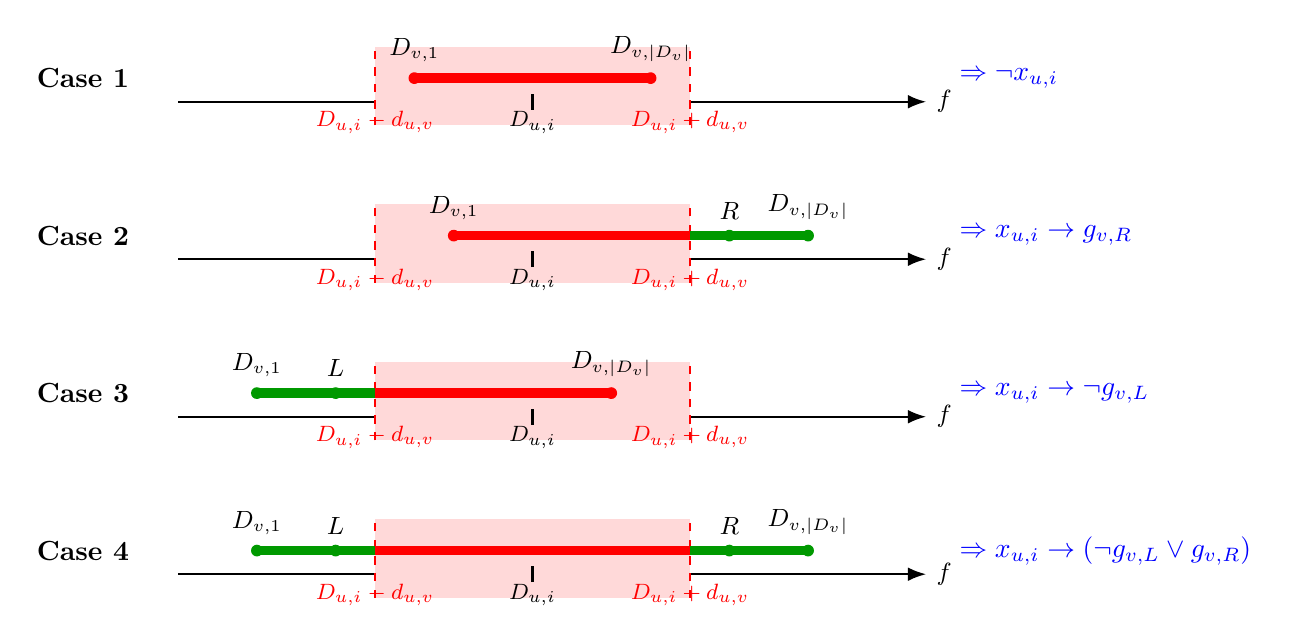
\begin{tikzpicture}[
    font=\small,
    axis/.style={-Latex, thick},
    forbidden/.style={fill=red!15},
    domain_invalid/.style={line width=3.5pt, red},
    domain_valid/.style={line width=3.5pt, green!60!black},
    domain_bound/.style={circle, fill, inner sep=1.5pt}
]

% Macros for repeated elements
\def\xCenter{4.5}
\def\d{2}
\def\fMin{\xCenter-\d} % 2.5
\def\fMax{\xCenter+\d} % 6.5

\newcommand{\drawBase}[2]{
    % Trục f
    \draw[axis] (0, #1) -- (9.5, #1) node[right] {$f$};
    % Vùng cấm màu đỏ
    \fill[forbidden] (\fMin, #1-0.3) rectangle (\fMax, #1+0.7);
    \draw[red, dashed, thick] (\fMin, #1-0.3) -- (\fMin, #1+0.7);
    \draw[red, dashed, thick] (\fMax, #1-0.3) -- (\fMax, #1+0.7);
    % Đánh dấu tâm D_{u,i} và giới hạn
    \draw[thick] (\xCenter, #1-0.1) -- (\xCenter, #1+0.1);
    \node[below, font=\footnotesize] at (\xCenter, #1) {$D_{u,i}$};
    \node[red, below, font=\footnotesize] at (\fMin, #1) {$D_{u,i}-d_{u,v}$};
    \node[red, below, font=\footnotesize] at (\fMax, #1) {$D_{u,i}+d_{u,v}$};
    % Tên Case
    \node[left, font=\bfseries] at (-0.5, #1+0.3) {#2};
}

% ==========================================
% Case 1: Dv nằm trọn trong vùng cấm (eq:forbid_1)
\drawBase{6}{Case 1}
\draw[domain_invalid] (3, 6.3) -- (6, 6.3);
\node[domain_bound, red, label=above:{$D_{v,1}$}] at (3, 6.3) {};
\node[domain_bound, red, label=above:{$D_{v,|D_v|}$}] at (6, 6.3) {};
\node[right, font=\bfseries, text=blue] at (9.8, 6.3) {$\Rightarrow \neg x_{u,i}$};

% ==========================================
% Case 2: Dv giao bên phải vùng cấm (eq:forbid_2)
\drawBase{4}{Case 2}
\draw[domain_invalid] (3.5, 4.3) -- (\fMax, 4.3);
\draw[domain_valid] (\fMax, 4.3) -- (8, 4.3);
\node[domain_bound, red, label=above:{$D_{v,1}$}] at (3.5, 4.3) {};
\node[domain_bound, green!60!black, label=above:{$D_{v,|D_v|}$}] at (8, 4.3) {};
\node[domain_bound, green!60!black, label=above:{$R$}] at (7, 4.3) {};
\node[right, font=\bfseries, text=blue] at (9.8, 4.3) {$\Rightarrow x_{u,i} \rightarrow g_{v,R}$};

% ==========================================
% Case 3: Dv giao bên trái vùng cấm (eq:forbid_3)
\drawBase{2}{Case 3}
\draw[domain_valid] (1, 2.3) -- (\fMin, 2.3);
\draw[domain_invalid] (\fMin, 2.3) -- (5.5, 2.3);
\node[domain_bound, green!60!black, label=above:{$D_{v,1}$}] at (1, 2.3) {};
\node[domain_bound, green!60!black, label=above:{$L$}] at (2, 2.3) {};
\node[domain_bound, red, label=above:{$D_{v,|D_v|}$}] at (5.5, 2.3) {};
\node[right, font=\bfseries, text=blue] at (9.8, 2.3) {$\Rightarrow x_{u,i} \rightarrow \neg g_{v,L}$};

% ==========================================
% Case 4: Dv trùm qua cả 2 bên vùng cấm (eq:forbid_4)
\drawBase{0}{Case 4}
\draw[domain_valid] (1, 0.3) -- (\fMin, 0.3);
\draw[domain_invalid] (\fMin, 0.3) -- (\fMax, 0.3);
\draw[domain_valid] (\fMax, 0.3) -- (8, 0.3);
\node[domain_bound, green!60!black, label=above:{$D_{v,1}$}] at (1, 0.3) {};
\node[domain_bound, green!60!black, label=above:{$L$}] at (2, 0.3) {};
\node[domain_bound, green!60!black, label=above:{$R$}] at (7, 0.3) {};
\node[domain_bound, green!60!black, label=above:{$D_{v,|D_v|}$}] at (8, 0.3) {};
\node[right, font=\bfseries, text=blue] at (9.8, 0.3) {$\Rightarrow x_{u,i} \rightarrow (\neg g_{v,L} \lor g_{v,R})$};

\end{tikzpicture}
\caption{Visualization of the 4 domain pruning scenarios based on Order Encoding. The forbidden frequency interval $[D_{u,i} - d_{u,v}, D_{u,i} + d_{u,v}]$ caused by assigning $x_{u,i} = \text{True}$ is highlighted in red. The valid sub-domains for neighbor $v$ are marked in green, enforced by boundary variables $g_{v,R}$ and $\neg g_{v,L}$.}
\label{fig:domain_pruning_cases}
\end{figure*}

Để làm rõ cơ chế hoạt động của hệ phương trình trên, Hình \ref{fig:domain_pruning_cases} minh họa trực quan 4 kịch bản tương tác giữa vùng cấm (màu đỏ) và miền tần số hợp lệ $D_v$ (màu xanh) của trạm kề. Thay vì phải sinh ra hàng loạt mệnh đề cấm $\neg x_{v,j}$ cho từng tần số đơn lẻ rơi vào vùng đỏ (như phương pháp Direct Encoding), mô hình PSE giải quyết bài toán bằng cách thiết lập các điểm neo biên (boundary points) $L$ và $R$.

Cụ thể, ở \textbf{Case 1} (Công thức \ref{eq:forbid_1}), khi toàn bộ miền $D_v$ bị "nuốt chửng" bởi vùng cấm, việc gán $x_{u,i} = \text{True}$ chắc chắn dẫn đến trạng thái vô nghiệm. Do đó, bộ giải lập tức sinh ra mệnh đề đơn (unit clause) $\neg x_{u,i}$ để loại bỏ rẽ nhánh này ngay từ đầu. Ở \textbf{Case 2} (\ref{eq:forbid_2}) và \textbf{Case 3} (\ref{eq:forbid_3}), khi $D_v$ chỉ có các tần số hợp lệ nằm lệch về một phía (phải hoặc trái), mô hình sử dụng phép kéo theo để ép trạm $v$ phải nhảy qua vùng cấm ($g_{v,R}$) hoặc lùi lại ranh giới an toàn ($\neg g_{v,L}$). Cuối cùng, phức tạp nhất là \textbf{Case 4} (\ref{eq:forbid_4}) khi miền $D_v$ trải dài qua cả hai bên vùng cấm. Lúc này, mệnh đề $(\neg g_{v,L} \lor g_{v,R})$ tạo ra một rẽ nhánh logic sắc bén: trạm $v$ bắt buộc phải chọn tần số ở dải an toàn bên trái hoặc dải an toàn bên phải. Bằng cách thiết lập các "bức tường" chặn bằng biến $g$, phương pháp PSE cho phép bộ giải tận dụng tối đa cơ chế lan truyền đơn vị (Unit Propagation) để cắt tỉa triệt để các khoảng vô nghiệm (holes) trong thời gian $O(1)$.

% \begin{align}
%     & \neg x_{u,j} \notag\\
%     & \forall(u, v, d_{u,v}) \in E \text{ s.t. } f_j - d_{u,v} \leq F_v(1) \wedge f_j + d_{u,v} \geq F_v(k)\\
%     & x_{u,j} \rightarrow g_{v,f_j+d_{u,v}+c} \forall(u, v, d_{u,v}) \in E \text{ s.t. }  f_j - d_{u,v} \leq F_v(1)\\
%     & x_{u,f_j} \rightarrow \neg y_{v,j-d_{u,v}+c} \forall(u, v, d_{u,v}) \in E \text{ s.t. } f_j + d_{u,v} \geq F_v(k)\\
%     & x_{u,f_j} \rightarrow \neg y_{v,fj-d_{u,v}+c} \vee y_{v,f_j+d_{u,v}+c} \forall(u, v, d_{u,v}) \in E \text{ s.t. } f_j - d_{u,v} > F_v(1) \wedge f_j + d_{u,v} < F_v(k)\\
%     &x_{u,f_j} \Leftrightarrow x_{v,f_j+d_{u,v}} \forall(u, v, d_{u,v}) \in E
% \end{align}

Ngoài ra, chính các Công thức \eqref{eq:g_right_bound}--\eqref{eq:g_propagation} cũng đã đảm bảo và thay thế cho Công thức \eqref{eq:sat_exact} của DSE.


\subsection{Objective Function Optimization via Incremental SAT}
\label{subsec:incremental_sat}
Sau khi không gian tìm kiếm cơ sở được thiết lập, mục tiêu của bài toán MO-FAP là cực tiểu hóa số lượng tần số phân biệt được sử dụng. Để theo dõi trạng thái của mạng lưới, gọi $D = \bigcup_{v \in V} D_v$ là tập hợp chứa toàn bộ các tần số khả dụng trong hệ thống, được sắp xếp tăng dần với kích thước $N = |D|$. Ta gọi $D_{j'}$ là giá trị tần số ở vị trí thứ $j'$ trong tập hợp này ($1 \le j' \le N$).

Khởi tạo tập biến Boolean trạng thái $A_{j'} \in \{\text{True}, \text{False}\}$, trong đó $A_{j'} = \text{True}$ khi và chỉ khi tần số $D_{j'}$ đang được sử dụng bởi ít nhất một thiết bị. Ràng buộc liên kết giữa cấu hình trạm và trạng thái tần số tổng thể được định nghĩa qua mệnh đề kéo theo trong Công thức \eqref{eq:active_link}. Hình \ref{fig:x_to_A_implication} minh họa một ví dụ cho liên kết này.
\begin{align}
    x_{v,j} \rightarrow A_{j'}, \quad \forall v \in V, \forall j, j' : D_{v,j} = D_{j'} \label{eq:active_link}
\end{align}

\begin{figure*}[htbp]
\centering
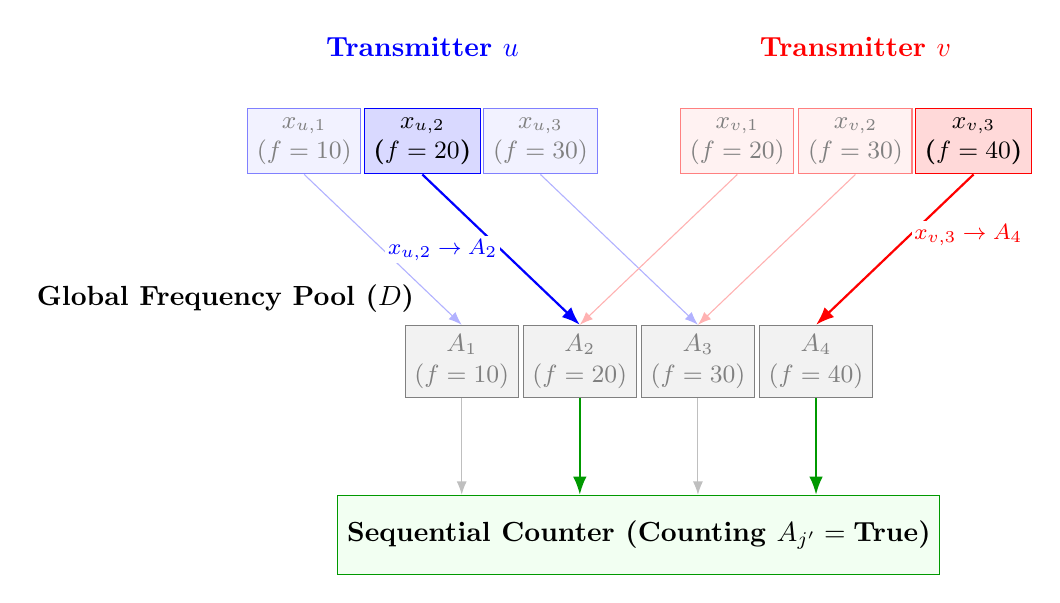
\begin{tikzpicture}[
    node distance = 1.5cm and 1cm,
    var_box/.style = {draw, rectangle, minimum width=1.2cm, minimum height=0.8cm, align=center, font=\small},
    % Style cho Trạm u (Màu Xanh)
    active_u/.style = {var_box, draw=blue, fill=blue!15, font=\small\bfseries},
    inactive_u/.style = {var_box, draw=blue!50, fill=blue!5, text=gray},
    arrow_u/.style = {-Latex, thick, blue},
    % Style cho Trạm v (Màu Đỏ)
    active_v/.style = {var_box, draw=red, fill=red!15, font=\small\bfseries},
    inactive_v/.style = {var_box, draw=red!50, fill=red!5, text=gray},
    arrow_v/.style = {-Latex, thick, red},
    % Style cho Biến Toàn cục A (Màu Xanh Lá)
    active_A/.style = {var_box, draw=green!60!black, fill=green!15, font=\small\bfseries},
    inactive_A/.style = {var_box, draw=gray, fill=gray!10, text=gray},
    arrow_A/.style = {-Latex, thick, green!60!black}
]

% --- Lớp trên: Trạm u và Trạm v (Local Domains) ---
% Trạm u
\node[text=blue] (u_label) at (-1.5, 2.2) {\textbf{Transmitter $u$}};
\node[inactive_u] (xu1) at (-3, 1) {$x_{u,1}$\\($f=10$)};
\node[active_u] (xu2) at (-1.5, 1) {$x_{u,2}$\\($f=20$)}; % Chọn f=20
\node[inactive_u] (xu3) at (0, 1) {$x_{u,3}$\\($f=30$)};

% Trạm v
\node[text=red] (v_label) at (4, 2.2) {\textbf{Transmitter $v$}};
\node[inactive_v] (xv1) at (2.5, 1) {$x_{v,1}$\\($f=20$)};
\node[inactive_v] (xv2) at (4, 1) {$x_{v,2}$\\($f=30$)};
\node[active_v] (xv3) at (5.5, 1) {$x_{v,3}$\\($f=40$)}; % Chọn f=40

% --- Lớp giữa: Global Frequency Pool (Các biến A) ---
\node (global_label) at (-4, -1) {\textbf{Global Frequency Pool ($D$)}};
\node[inactive_A] (A1) at (-1, -1.8) {$A_1$\\($f=10$)};
\node[inactive_A] (A2) at (0.5, -1.8) {$A_2$\\($f=20$)};
\node[inactive_A] (A3) at (2, -1.8) {$A_3$\\($f=30$)};
\node[inactive_A] (A4) at (3.5, -1.8) {$A_4$\\($f=40$)};

% --- Vẽ mũi tên lan truyền (Implications) ---
% Từ Trạm u (Màu Xanh Dương)
\draw[-Latex, draw=blue!30] (xu1.south) -- (A1.north);
\draw[arrow_u] (xu2.south) -- node[left, pos=0.5, font=\footnotesize, fill=white, inner sep=1pt] {$x_{u,2} \rightarrow A_2$} (A2.north);
\draw[-Latex, draw=blue!30] (xu3.south) -- (A3.north);

% Từ Trạm v (Màu Đỏ)
\draw[-Latex, draw=red!30] (xv1.south) -- (A2.north);
\draw[-Latex, draw=red!30] (xv2.south) -- (A3.north);
\draw[arrow_v] (xv3.south) -- node[right, pos=0.4, font=\footnotesize, fill=white, inner sep=1pt] {$x_{v,3} \rightarrow A_4$} (A4.north);

% --- Lớp dưới: Sequential Counter ---
\node[draw=green!60!black, rectangle, minimum width=6cm, minimum height=1cm, fill=green!5, font=\bfseries] (counter) at (1.25, -4) {Sequential Counter (Counting $A_{j'} = \text{True}$)};

% Mũi tên từ A xuống Counter
\draw[-Latex, draw=gray!50] (A1.south) -- (A1.south |- counter.north);
\draw[arrow_A] (A2.south) -- (A2.south |- counter.north);
\draw[-Latex, draw=gray!50] (A3.south) -- (A3.south |- counter.north);
\draw[arrow_A] (A4.south) -- (A4.south |- counter.north);

\end{tikzpicture}
\caption{Illustration of the implication mechanism ($x_{v,j} \rightarrow A_{j'}$) linking local frequency assignments to global active frequencies.}
\label{fig:x_to_A_implication}
\end{figure*}

Quá trình tối ưu hóa hàm mục tiêu được thực hiện thông qua chiến lược tìm kiếm tuyến tính (Linear Search). Thuật toán bắt đầu bằng việc giải mô hình cơ sở để tìm một lời giải khả thi đầu tiên, qua đó xác lập cận trên $UB$ (Upper Bound) ban đầu cho số lượng tần số. Ở mỗi bước lặp tiếp theo, hệ thống bị ép phải tìm một cấu hình sử dụng tối đa $k = UB - 1$ tần số (ràng buộc At-Most-$k$). Nếu một cấu hình hợp lệ được tìm thấy, $UB$ được cập nhật bằng giá trị mới và vòng lặp tiếp tục cho đến khi bộ giải trả về \texttt{UNSAT}, chứng minh $UB$ hiện tại là mức tối ưu tuyệt đối.
Về mặt lý thuyết, các vòng lặp tìm kiếm này hoàn toàn có thể được thực thi như những phiên giải SAT độc lập (independent solver calls). Nghĩa là, ở mỗi giới hạn $k$ mới, ta lại khởi tạo một bộ giải mới, xây dựng lại toàn bộ tập mệnh đề từ đầu và tiến hành giải. Tuy nhiên, cách làm này cực kỳ kém hiệu quả vì nó bắt buộc bộ giải phải khởi động lại (restart), làm xóa sạch toàn bộ không gian trạng thái và các mệnh đề học được (learned clauses) quý giá đã tích lũy từ những vòng lặp trước. Để tối ưu hóa quá trình này, chúng tôi áp dụng kỹ thuật SAT tăng cường (Incremental SAT) \cite{martins2014incremental}, cho phép tái sử dụng bộ giải đang chạy qua nhiều vòng lặp. Trong khuôn khổ Incremental SAT, có hai cách tiếp cận để áp đặt giới hạn số tần số được sử dụng như sau:

\textbf{Cách tiếp cận ngây thơ (Naive Incremental Approach):} 
Trong các phương pháp Incremental thông thường, mỗi khi cận trên $UB$ giảm xuống, một tập hợp các biến phụ và mệnh đề At-Most-$k$ mới sẽ được sinh ra và bổ sung trực tiếp vào bộ giải. Việc liên tục thêm mới công thức qua từng vòng lặp không chỉ dẫn đến tình trạng phình to bộ nhớ và tiêu tốn chi phí thời gian khởi tạo biến và mệnh đề mới, mà còn làm tăng độ phức tạp của không gian tìm kiếm, qua đó làm suy giảm đáng kể tốc độ hội tụ của bộ giải SAT.


\textbf{Phương pháp đề xuất (Proposed Incremental Approach):} 
Để khắc phục triệt để chi phí tái khởi tạo, chúng tôi đề xuất một cơ chế tối ưu kết hợp mã hóa bộ đếm tuần tự (Sequential Counter - Sinz, 2005) và kỹ thuật SAT tăng cường (Incremental SAT). Điểm đột phá của phương pháp này là bộ đếm chỉ được khởi tạo duy nhất một lần với cận trên ban đầu $UB$. 

Cụ thể, tập biến phụ $S_{j',c}$ ($1 \le j' \le N, 1 \le c \le UB$) được sinh ra mang ý nghĩa: trong $j'$ tần số đầu tiên, có ít nhất $c$ tần số ở trạng thái kích hoạt. Khối mệnh đề logic của bộ đếm được thiết lập cố định bởi các Công thức \eqref{eq:nsc_1}--\eqref{eq:nsc_7}:

Nếu kết quả trả về \texttt{SAT}, một giới hạn $UB'$ mới được ghi nhận, giả định cũ bị gỡ bỏ trong thời gian $O(1)$ và vòng lặp tiếp theo được gọi với giả định $\neg S_{N, UB'}$. Vòng lặp này sẽ diễn ra liên tục cho đến khi kết quả trả về từ bộ giải SAT là \texttt{SAT} hoặc bị ngắt bởi giới hạn về thời gian hoặc bộ nhớ. Chiến lược truyền \textit{Assumptions} này giúp công thức không bị phình to qua các vòng lặp, đồng thời cho phép bộ giải duy trì nguyên vẹn cây tìm kiếm và tận dụng 100\% tri thức từ các mệnh đề học được. Nhờ đó, phương pháp đề xuất loại bỏ hoàn toàn chi phí (overhead) của việc tái cấu trúc bộ đếm, đẩy nhanh đáng kể tốc độ hội tụ so với cách tiếp cận khởi động lại truyền thống.

\begin{align}
    &\bigwedge_{i=1}^{n}
    \left( A_i \rightarrow S_{i,1} \right)
    \label{eq:nsc_1}
    && \\
    &\bigwedge_{i=2}^{n}
    \;\bigwedge_{j=1}^{\min(i-1,k)}
    \left( S_{i-1,j} \rightarrow S_{i,j} \right)
    \label{eq:nsc_2}
    && \\
    &\bigwedge_{i=2}^{n}
    \;\bigwedge_{j=2}^{\min(i,k)}
    \left( A_i \land S_{i-1,j-1} \rightarrow S_{i,j} \right)
    \label{eq:nsc_3}
    && \\
    &\bigwedge_{i=2}^{n}
    \;\bigwedge_{j=1}^{\min(i-1,k)}
    \left( \neg A_i \land \neg S_{i-1,j} \rightarrow \neg S_{i,j} \right)
    \label{eq:nsc_4}
    && \\
    &\bigwedge_{i=1}^{k}
    \left( \neg A_i \rightarrow \neg S_{i,i} \right)
    \label{eq:nsc_5}
    && \\
    &\bigwedge_{i=2}^{n}
    \;\bigwedge_{j=2}^{\min(i,k)}
    \left( \neg S_{i-1,j-1} \rightarrow \neg S_{i,j} \right)
    \label{eq:nsc_6}
    && \\
    &\bigwedge_{i=k+1}^{n}
    \left( A_i \rightarrow \neg S_{i-1,k} \right)
    \label{eq:nsc_7}
    && \\
\end{align}

% Với cấu trúc mạch logic này, biến $S_{N, k+1}$ ở cuối chuỗi sẽ mang giá trị True nếu mạng lưới sử dụng vượt quá $k$ tần số. Do đó, để áp đặt điều kiện At-Most-$k$, thay vì sinh thêm mệnh đề mới, chúng tôi khai thác cơ chế \textit{Assumptions} của bộ giải Cadical (thông qua giao diện \texttt{PySAT.Solvers}). Ở mỗi vòng lặp với mục tiêu tối đa $k$ tần số, thuật toán chỉ truyền trực tiếp một giả định duy nhất là $\neg S_{N, k+1}$ vào lời gọi hàm \texttt{solve()}. Giả định này đóng vai trò như một quyết định tạm thời ở cấp độ gốc của cây tìm kiếm (root-level decision). 


\subsection{Experimental Setup}
\label{sec:exp}
Toàn bộ thực nghiệm được tiến hành trên hệ thống máy tính trang bị bộ vi xử lý Intel Core i7-10850H và 16 GB RAM, vận hành trên nền tảng hệ điều hành Ubuntu 24.04.3 LTS. Quá trình giải quyết các bài toán SAT được thực thi bởi bộ giải CaDiCaL (phiên bản 1.9.5) thông qua giao diện lập trình ứng dụng (API) của thư viện \texttt{PySAT} \cite{imms-sat18,itk-sat24}. 

Nhằm kiểm soát chặt chẽ và giám sát chính xác mức độ tiêu thụ tài nguyên của các thuật toán, chúng tôi tích hợp công cụ \texttt{runlim}\footnote{\url{https://github.com/arminbiere/runlim/}}. Đối với mỗi phiên giải (solver instance), hệ thống áp đặt một giới hạn nghiêm ngặt: thời gian thực thi tối đa (Time Limit) là 600 giây và giới hạn bộ nhớ (Memory Limit) được cấp phát tối đa là 14.000 MB. Bất kỳ tiến trình nào vượt qua các ngưỡng này đều bị hệ thống buộc dừng và ghi nhận kết quả tương ứng là Timeout (TL) hoặc Out of Memory (OOM).

Các thực nghiệm được tiến hành trên hai bộ dữ liệu tiêu chuẩn là CALMA và DUTtest, vốn đã được kiểm chứng rộng rãi trong các nghiên cứu trước đây (được lưu trữ tại cơ sở dữ liệu FAP web\footnote{\url{https://fap.zib.de/}}). Đối với bộ CALMA, bên cạnh các kịch bản (instances) vốn đã được thiết kế sẵn cho bài toán tối ưu số lượng tần số (MO-FAP), chúng tôi cũng mở rộng không gian đánh giá bằng cách tái định dạng (reformulate) hàm mục tiêu của tất cả các instance còn lại về dạng cực tiểu hóa số lượng tần số sử dụng. Bảng \ref{tab:calma} tóm tắt các đặc trưng cấu trúc của bộ dữ liệu CALMA, trong đó $|V|$ và $|E|$ lần lượt biểu diễn số lượng thiết bị thu phát và số lượng ràng buộc khoảng cách của mạng lưới.

\begin{table}[ht]
\centering
\caption{Characteristics of CALMA benchmark instances}
\label{tab:calma}
\begin{tabular}{l l r r}
\hline
\textbf{Instance} & \textbf{Original Objective} & $|V|$ & $|E|$ \\
\hline
CELAR 01 & Minimum Order        & 916 & 5548 \\
CELAR 02 & Minimum Order        & 200 & 1235 \\
CELAR 03 & Minimum Order        & 400 & 2760 \\
CELAR 04 & Minimum Order        & 680 & 3967 \\
CELAR 05 & Minimum Span         & 400 & 2598 \\
CELAR 06 & Minimum Interference & 200 & 1322 \\
CELAR 07 & Minimum Interference & 400 & 2865 \\
CELAR 08 & Minimum Interference & 916 & 5744 \\
CELAR 09 & Minimum Interference & 680 & 4103 \\
CELAR 10 & Minimum Interference & 680 & 4103 \\
CELAR 11 & Minimum Order        & 680 & 4103 \\
GRAPH 01 & Minimum Order        & 200 & 1134 \\
GRAPH 02 & Minimum Order        & 400 & 2245 \\
GRAPH 03 & Minimum Span         & 200 & 1134 \\
GRAPH 04 & Minimum Span         & 400 & 2244 \\
GRAPH 05 & Minimum Interference & 200 & 1134 \\
GRAPH 06 & Minimum Interference & 400 & 2170 \\
GRAPH 07 & Minimum Interference & 400 & 2170 \\
GRAPH 08 & Minimum Order        & 680 & 3757 \\
GRAPH 09 & Minimum Order        & 916 & 5246 \\
GRAPH 10 & Minimum Span         & 680 & 3907 \\
GRAPH 11 & Minimum Interference & 680 & 3757 \\
GRAPH 12 & Minimum Interference & 680 & 4017 \\
GRAPH 13 & Minimum Interference & 916 & 5273 \\
GRAPH 14 & Minimum Order        & 916 & 4638 \\
\hline
\end{tabular}
\end{table}

Nhằm đánh giá một cách toàn diện và khách quan hiệu năng của mô hình, chúng tôi thiết lập một hệ thống đối sánh đa chiều. Đầu tiên, phương pháp mã hóa đề xuất (Proposed SAT Encoding) được đối chiếu trực tiếp với mô hình mã hóa cơ sở (Direct SAT Encoding) nhằm làm rõ tính hiệu quả của kỹ thuật cắt tỉa miền giá trị. Tiếp theo, sức mạnh tổng thể của hệ thống được đặt lên bàn cân với các phần mềm tối ưu hóa thương mại hàng đầu hiện nay, cụ thể là các bộ giải Quy hoạch nguyên hỗn hợp (MIP)\cite{} và Lập trình ràng buộc (CP)\cite{} được cung cấp bởi Gurobi (v13.0.0)\footnote{\url{https://www.gurobi.com}} và IBM ILOG CPLEX (v12.1.1)\footnote{\url{https://www.ibm.com/products/ilog-cplex-optimization-studio}}. Cuối cùng, để khẳng định chất lượng và độ tin cậy của các nghiệm tìm được, kết quả thực nghiệm sẽ được tham chiếu chéo với các giới hạn tối ưu (bounds) tốt nhất từ các nghiên cứu trước đây.

Để chuẩn hóa việc trình bày kết quả, các ký hiệu sau được sử dụng để định nghĩa các thành phần thuật toán: \textbf{DSE} và \textbf{POSE} lần lượt là mô hình \textit{Direct SAT Encoding} và \textit{Proposed Order-based SAT Encoding}; \textbf{INC} là chiến lược \textit{Naive Incremental Approach} của hàm mục tiêu, trong khi \textbf{INCSC} là chiến lược hàm mục tiêu đề xuất sử dụng Sequential Counter (\textit{Proposed Incremental Ap-
proach}). Các bộ giải baseline được ký hiệu là \textbf{Gurobi}, \textbf{CPLEX-MIP} và \textbf{CPLEX-CP}. 
Một phương pháp SAT hoàn chỉnh được ký hiệu bằng cách ghép tên phương pháp mã hóa với tên chiến lược hàm mục tiêu (Ví dụ \textbf{POSE+INCSC}).

\subsection{Evaluation of Domain Preprocessing}

Bảng \ref{tab:preprocess_stats} thể hiện hiệu quả khi áp dụng Domain Preprocessing trên 35 instance thông qua ba tiêu chí: số instance cải thiện chất lượng nghiệm hoặc không bị dừng bởi giới hạn tài nguyên so với khi chưa áp dụng Domain Preprocessing (\textit{Better Sol.}), số instance có cùng chất lượng lời giải nhưng thời gian giải nhanh hơn  (\textit{Faster Time}). Ngoài ra, \textit{INF} là để chỉ các instance cho lời giải vô nghiệm (Infeasible). Dữ liệu thực nghiệm chỉ ra rằng, tiền xử lý không chỉ giúp các hệ thống SAT tăng tốc độ giải (nhanh hơn tới 71.43\% đối với \textbf{POSE+INCSC}), mà còn tăng tốc cho cả các bộ giải thương mại. Cụ thể, kỹ thuật này cứu \textbf{CPX-MIP} và \textbf{CPX-CP} thoát khỏi giới hạn tài nguyên (\texttt{TO}/\texttt{OOM}) để giải thành công lần lượt 7 và 6 instance. Đặc biệt, sự cải thiện thời gian thể hiện sự áp đảo tại 13 instance \texttt{INF}; thay vì cố gắng tìm kiếm một lời giải không tồn tại. Sự thu hẹp miền giá trị $D$ của các đỉnh đã giúp chứng minh trạng thái \texttt{UNSAT} gần như tức thời. Như vậy, việc đánh đổi một phần nhỏ chi phí thời gian khởi tạo ở các đồ thị lỏng lẻo là hoàn toàn xứng đáng để cấu trúc hóa không gian tìm kiếm và đảm bảo tính ổn định vững chắc cho hệ thống.

\begin{table}[H]
\centering
\caption{Impact of Pre-processing on 35 benchmark instances}
\label{tab:preprocess_stats}
\begin{tabular}{l|c|c|c}
\toprule
\textbf{Solver} & \textbf{Better Sol.\textsuperscript{a}} & \textbf{Faster Time\textsuperscript{b}} & \textbf{Total\textsuperscript{c}} \\ 
\midrule
POSE+INCSC & 0 & 25 (71.43\%) & 25 (13 INF) \\
POSE+INC   & 0 & 24 (68.57\%) & 24 (13 INF) \\
DSE        & 0 & 22 (62.86\%) & 22 (13 INF) \\
GUR        & 1 & 25 (78.12\%) & 26 (13 INF) \\
CPX-CP     & 6 & 13 (54.17\%) & 19 (13 INF) \\
CPX-MIP    & 7 & 13 (54.17\%) & 20 (11 INF) \\
\bottomrule
\multicolumn{4}{l}{\footnotesize \textsuperscript{a} Smaller objective value or successfully escaping Timeout/OOM limits.} \\
\multicolumn{4}{l}{\footnotesize \textsuperscript{b} Faster execution time when both yield the same objective value.} \\
\multicolumn{4}{l}{\footnotesize \textsuperscript{c} Total improvements (INF instances shown in parentheses).}
\end{tabular}
\end{table}



\subsection{Evaluation of the Proposed Encoding for Distance Constraint}

\begin{table}[htbp]
\centering
\caption{Comparison of Distance Encodings: Proposed SAT Encoding (POSE) vs. Direct SAT Encoding (DSE)}
\label{tab:pose_vs_dse}
\begin{tabular}{l c c r r c c}
\toprule
\textbf{Instance} & \multicolumn{2}{c}{\textbf{Solution}} & \multicolumn{2}{c}{\textbf{Total Time (s)}} & \multicolumn{2}{c}{\textbf{Status}} \\
\cmidrule(lr){2-3} \cmidrule(lr){4-5} \cmidrule(lr){6-7}
 & \textbf{POSE} & \textbf{DSE} & \textbf{POSE} & \textbf{DSE} & \textbf{POSE} & \textbf{DSE} \\
\midrule
C01 & 16 & - & \textbf{106.02} & TO & OPT & TO \\
C02 & 14 & - & \textbf{14.63} & TO & OPT & TO \\
C03 & 14 & - & \textbf{68.84} & TO & OPT & TO \\
C04 & 46 & 46 & \textbf{0.06} & 0.11 & OPT & OPT \\
C05 & 40 & 40 & \textbf{0.29} & 0.54 & OPT & OPT \\
C06 & - & - & \textbf{0.19} & 0.39 & INF & INF \\
C07 & - & - & \textbf{0.30} & 0.60 & INF & INF \\
C08 & - & - & \textbf{0.69} & 1.37 & INF & INF \\
C09 & - & - & 0.01 & 0.01 & INF & INF \\
C10 & - & - & 0.01 & 0.01 & INF & INF \\
C11 & 22 & - & \textbf{29.21} & TO & OPT & TO \\
G01 & 18 & - & \textbf{76.26} & TO & OPT & TO \\
G02 & 14 & - & \textbf{12.17} & TO & OPT & TO \\
G03 & 20 & 20 & \textbf{5.88} & 7.25 & OPT & OPT \\
G04 & 22 & 22 & \textbf{13.13} & 23.07 & OPT & OPT \\
G05 & - & - & \textbf{0.04} & 0.05 & INF & INF \\
G06 & - & - & \textbf{0.23} & 0.43 & INF & INF \\
G07 & - & - & 0.01 & 0.01 & INF & INF \\
G08 & 18 & - & \textbf{17.67} & TO & OPT & TO \\
G09 & 18 & - & \textbf{61.55} & TO & OPT & TO \\
G10 & 22 & 22 & \textbf{33.63} & 248.49 & OPT & OPT \\
G11 & - & - & \textbf{0.43} & 0.89 & INF & INF \\
G12 & - & - & 0.01 & 0.01 & INF & INF \\
G13 & - & - & TO & TO & TO & TO \\
G14 & 8 & 8 & \textbf{10.16} & 13.35 & OPT & OPT \\
TUD200.1 & 12 & 12 & \textbf{3.34} & 67.88 & OPT & OPT \\
TUD200.2 & 46 & 46 & \textbf{0.10} & 0.19 & OPT & OPT \\
TUD200.3 & 14 & 14 & \textbf{1.45} & 1.95 & OPT & OPT \\
TUD200.4 & 20 & 20 & \textbf{0.10} & 0.17 & OPT & OPT \\
TUD200.5 & - & - & \textbf{0.13} & 0.25 & INF & INF \\
TUD916.1 & 18 & 18 & \textbf{9.77} & 17.00 & OPT & OPT \\
TUD916.2 & 48 & 48 & \textbf{0.41} & 0.68 & OPT & OPT \\
TUD916.3 & 24 & 24 & 3.31 & \textbf{2.65} & OPT & OPT \\
TUD916.4 & 26 & 26 & \textbf{0.50} & 0.92 & OPT & OPT \\
TUD916.5 & - & - & 0.21 & 0.21 & INF & INF \\
\bottomrule
\multicolumn{7}{l}{\footnotesize \textbf{OPT}: Optimal, \textbf{INF}: Infeasible, \textbf{TO}: Timeout (600s).} \\
\multicolumn{7}{l}{\footnotesize Bold values indicate the faster execution time.}
\end{tabular}
\end{table}


% Hàm distance so: Cái của mình, Pairwise
% Hàm mục tiêu: Dùng chung nsc\_assumptions
Mục tiêu của thực nghiệm này là đánh giá độc lập hiệu năng của mô hình phương pháp mã hóa đề xuất (\textbf{POSE}) so với phương pháp mã hóa trực tiếp (\textbf{DSE}). Để đảm bảo công bằng, cả hai cấu hình đều được áp dụng Domain preprocessing và chiến lược tối ưu hàm mục tiêu \textit{INCSC}. Chi tiết đối sánh trên 35 instance được trình bày tại Bảng \ref{tab:pose_vs_dse}, trong đó trạng thái kết thúc của bộ giải được phân định thành ba nhóm: \texttt{OPT} (tìm thấy và chứng minh được nghiệm tối ưu), \texttt{INF} (chứng minh cấu trúc bài toán vô nghiệm), và \texttt{TO} (cạn kiệt giới hạn thời gian 600 giây mà không thể kết luận).

Dữ liệu thực nghiệm phản ánh sự vượt trội toàn diện của \textbf{POSE} về thời gian giải cũng như khả năng hội tụ so với mã hóa trực tiếp. Cụ thể, \textbf{POSE} giải quyết thành công 34/35 instance trong giới hạn 600 giây (chỉ duy nhất \texttt{G13} cạn kiệt thời gian). Ngược lại, việc biểu diễn không gian bằng các biến boolean rời rạc khiến \textbf{DSE} gặp hiện tượng bùng nổ tổ hợp và cạn kiệt tài nguyên (\texttt{TO}) tại 9 instance. Đáng chú ý, có tới 8 instance khắt khe (điển hình như chuỗi \texttt{C01-C03, C11} và \texttt{G01, G02, G08, G09}) mà \textbf{DSE} hoàn toàn bất lực (\texttt{TO}), trong khi \textbf{POSE} vẫn xuất sắc tìm ra và chứng minh được nghiệm tối ưu (\texttt{OPT}). Ngay cả trên các instance mà \textbf{DSE} có khả năng hội tụ, \textbf{POSE} vẫn duy trì tốc độ xử lý nhanh hơn từ hàng chục đến hàng trăm lần, tiêu biểu như ở instance \texttt{TUD200.1} ($3.34$s so với $67.88$s) hay \texttt{G10} ($33.63$s so với $248.49$s).

Sức mạnh cấu trúc của mã hóa đề xuất tiếp tục được bộc lộ sắc nét qua các infeasible instance(\texttt{INF}). Để kết luận một hệ thống là \texttt{INF}, bộ giải buộc phải duyệt và cắt tỉa toàn bộ không gian tìm kiếm. Kết quả cho thấy \textbf{POSE} chạm đến giới hạn \texttt{UNSAT} nhanh hơn (hoặc tương đương ở các ca cực nhỏ) so với \textbf{DSE} trong 100\% các bài test. Sự chênh lệch này là minh chứng vững chắc cho sự hiệu quả của phương pháp mã hóa khoảng các đề xuất \textbf{POSE} với các biến $g$ đã được xây dựng. 

\subsection{Evaluation of the Objective Function Optimization}
% Hàm distance: Dùng chung cái của mình
% Hàm mục tiêu: nsc\_assumptions vs tot\_assumption
\begin{table}[htbp]
\centering
\caption{Comparison of Incremental Strategies: Proposed INCSC vs. Basic INC}
\label{tab:inc_vs_incsc}
\begin{tabular}{l c r r c c}
\toprule
\textbf{Instance} & \textbf{Solution} & \multicolumn{2}{c}{\textbf{Total Time (s)}} & \multicolumn{2}{c}{\textbf{Status}} \\
\cmidrule(lr){3-4} \cmidrule(lr){5-6}
 &  & \textbf{INCSC} & \textbf{INC} & \textbf{INCSC} & \textbf{INC} \\
\midrule
C01 & 16 & \textbf{106.02} & 169.61 & OPT & OPT \\
C02 & 14 & \textbf{14.63} & 22.26 & OPT & OPT \\
C03 & 14 & \textbf{68.84} & 102.50 & OPT & OPT \\
C04 & 46 & 0.06 & 0.06 & OPT & OPT \\
C05 & 40 & 0.29 & 0.29 & OPT & OPT \\
C06 & - & 0.19 & 0.19 & INF & INF \\
C07 & - & 0.30 & 0.30 & INF & INF \\
C08 & - & 0.69 & \textbf{0.68} & INF & INF \\
C09 & - & 0.01 & 0.01 & INF & INF \\
C10 & - & 0.01 & 0.01 & INF & INF \\
C11 & 22 & 29.21 & \textbf{26.43} & OPT & OPT \\
G01 & 18 & \textbf{76.26} & 120.11 & OPT & OPT \\
G02 & 14 & \textbf{12.17} & 24.00 & OPT & OPT \\
G03 & 20 & 5.88 & \textbf{5.62} & OPT & OPT \\
G04 & 22 & 13.13 & \textbf{9.60} & OPT & OPT \\
G05 & - & 0.04 & 0.04 & INF & INF \\
G06 & - & 0.23 & 0.23 & INF & INF \\
G07 & - & 0.01 & 0.01 & INF & INF \\
G08 & 18 & \textbf{17.67} & 33.83 & OPT & OPT \\
G09 & 18 & \textbf{61.55} & 87.17 & OPT & OPT \\
G10 & 22 & 33.63 & \textbf{30.28} & OPT & OPT \\
G11 & - & 0.43 & \textbf{0.42} & INF & INF \\
G12 & - & 0.01 & 0.01 & INF & INF \\
G13 & - & 0.62 & 0.62 & OPT & OPT \\
G14 & 8 & \textbf{10.16} & 13.93 & OPT & OPT \\
TUD200.1 & 12 & \textbf{3.34} & 6.57 & OPT & OPT \\
TUD200.2 & 46 & 0.10 & 0.10 & OPT & OPT \\
TUD200.3 & 14 & \textbf{1.45} & 1.47 & OPT & OPT \\
TUD200.4 & 20 & 0.10 & 0.10 & OPT & OPT \\
TUD200.5 & - & 0.13 & 0.13 & INF & INF \\
TUD916.1 & 18 & \textbf{9.77} & 14.60 & OPT & OPT \\
TUD916.2 & 48 & 0.41 & \textbf{0.40} & OPT & OPT \\
TUD916.3 & 24 & 3.31 & \textbf{3.24} & OPT & OPT \\
TUD916.4 & 26 & 0.50 & \textbf{0.49} & OPT & OPT \\
TUD916.5 & - & 0.21 & 0.21 & INF & INF \\
\bottomrule
\multicolumn{6}{l}{\footnotesize \textbf{OPT}: Optimal, \textbf{INF}: Infeasible, \textbf{TO}: Timeout (600s).} \\
\multicolumn{6}{l}{\footnotesize Bold values indicate the faster execution time.}
\end{tabular}
\end{table}

Thực nghiệm này so sánh hiệu năng giữa chiến lược tối ưu tiệm tiến đề xuất (\textbf{INCSC}) và chiến lược tiệm tiến cơ bản (\textbf{INC}) trên nền tảng mã hóa \textbf{POSE}. Kết quả chi tiết tại Bảng \ref{tab:inc_vs_incsc} cho thấy mặc dù cả hai phương pháp đều bảo toàn tính tối ưu và hội tụ về cùng một giá trị mục tiêu (\textit{Solution}), \textbf{INCSC} thể hiện ưu thế rõ rệt về tốc độ xử lý trên các instance có không gian tìm kiếm lớn hoặc cấu trúc ràng buộc phức tạp. 

Cụ thể, đối với các instance khó như chuỗi \texttt{C01-C03} và \texttt{G01-G02}, \textbf{INCSC} giúp rút ngắn thời gian giải từ 30\% đến 50\% so với \textbf{INC}. Sự bứt phá này xuất phát từ khả năng tái sử dụng các biến và mệnh đề cũ. Trong khi \textbf{INCSC} chỉ cần thêm một tập mệnh đề ``at\_most\_k'' trong lần lặp đầu tiên và chỉ phải thêm một mệnh đề trong các lần lặp tiếp theo thì \textbf{INC} lại tốn thời gian thêm từng tập mệnh đề ``at\_most\_k'' trong tất cả các lần lặp. Như vậy, \textbf{INCSC} đã tiết kiệm được về cả thời gian thêm các biến và mệnh đề lẫn thời gian để bộ giải xử lý các mệnh đề đó.
% Sự bứt phá này xuất phát từ cơ chế thay đổi chiến lược linh hoạt (Strategy Change), cho phép bộ giải "nhảy vọt" qua các phân vùng không gian không chứa nghiệm thay vì phải kiểm tra từng mức giá trị hàm mục tiêu một cách tuần tự như \textbf{INC}. 
Ở các instance quy mô nhỏ hoặc trạng thái vô nghiệm (\texttt{INF}), thời gian giải của hai phương pháp là tương đương do số lượng bước lặp tiệm tiến không đáng kể. Kết quả này minh chứng rằng \textbf{INCSC} tối ưu hơn \textbf{INC} rất nhiều về mặt thời gian nhưng vẫn giữ nguyên được chất lượng lời giải.


\subsection{Comparison with State-of-the-Art Exact Solvers}

\begin{table*}[htbp]
\centering
\caption{Comprehensive Comparison between Proposed POSE+INCSC and SOTA Solvers}
\label{tab:super_master}
\resizebox{\textwidth}{!}{%
\begin{tabular}{l ccc ccc ccc ccc}
\toprule
\textbf{Instance} & \multicolumn{3}{c}{\textbf{Proposed}} & \multicolumn{3}{c}{\textbf{Gurobi}} & \multicolumn{3}{c}{\textbf{CPLEX-CP}} & \multicolumn{3}{c}{\textbf{CPLEX-MIP}} \\
\cmidrule(lr){2-4} \cmidrule(lr){5-7} \cmidrule(lr){8-10} \cmidrule(lr){11-13}
 & \textbf{Solution} & \textbf{Total Time (s)} & \textbf{Status} & \textbf{Solution} & \textbf{Total Time (s)} & \textbf{Status} & \textbf{Solution} & \textbf{Total Time (s)} & \textbf{Status} & \textbf{Solution} & \textbf{Total Time (s)} & \textbf{Status} \\
\midrule
C01 & 16 & \textbf{106.02} & OPT & - & TO & TO & - & TO & TO & - & TO & TO \\
C02 & 14 & 14.63 & OPT & 14 & \textbf{2.80} & OPT & - & TO & TO & 14 & 22.26 & OPT \\
C03 & 14 & \textbf{68.84} & OPT & - & TO & TO & - & TO & TO & - & TO & TO \\
C04 & 46 & \textbf{0.06} & OPT & 46 & 0.16 & OPT & 46 & 0.59 & OPT & 46 & 0.71 & OPT \\
C05 & 40 & \textbf{0.29} & OPT & 40 & 3.81 & OPT & 40 & 450.52 & OPT & 40 & 77.41 & OPT \\
C06 & - & \textbf{0.19} & INF & - & 3.31 & INF & - & 31.32 & INF & - & 45.71 & INF \\
C07 & - & \textbf{0.30} & INF & - & 4.37 & INF & - & 18.07 & INF & - & TO & TO \\
C08 & - & \textbf{0.69} & INF & - & 9.72 & INF & - & 85.17 & INF & - & TO & TO \\
C09 & - & \textbf{0.01} & INF & - & 0.02 & INF & - & \textbf{0.01} & INF & - & \textbf{0.01} & INF \\
C10 & - & \textbf{0.01} & INF & - & \textbf{0.01} & INF & - & \textbf{0.01} & INF & - & \textbf{0.01} & INF \\
C11 & 22 & \textbf{29.21} & OPT & 22 & 69.45 & OPT & - & TO & TO & 22 & 461.00 & OPT \\
G01 & 18 & 76.26 & OPT & 18 & \textbf{1.96} & OPT & - & TO & TO & 18 & 7.75 & OPT \\
G02 & 14 & 12.17 & OPT & 14 & \textbf{5.32} & OPT & - & TO & TO & 14 & 35.95 & OPT \\
G03 & 20 & \textbf{5.88} & OPT & - & TO & TO & - & TO & TO & - & TO & TO \\
G04 & 22 & \textbf{13.13} & OPT & - & TO & TO & - & TO & TO & - & TO & TO \\
G05 & - & \textbf{0.04} & INF & - & \textbf{0.04} & INF & - & \textbf{0.04} & INF & - & \textbf{0.04} & INF \\
G06 & - & \textbf{0.23} & INF & - & 2.44 & INF & - & 7.28 & INF & - & 59.23 & INF \\
G07 & - & \textbf{0.01} & INF & - & \textbf{0.01} & INF & - & \textbf{0.01} & INF & - & \textbf{0.01} & INF \\
G08 & 18 & 17.67 & OPT & 18 & \textbf{17.43} & OPT & - & TO & TO & - & TO & TO \\
G09 & 18 & \textbf{61.55} & OPT & 18 & 70.89 & OPT & - & TO & TO & - & TO & TO \\
G10 & 22 & \textbf{33.63} & OPT & - & TO & TO & - & TO & TO & - & TO & TO \\
G11 & - & \textbf{0.43} & INF & - & 5.14 & INF & - & 16.18 & INF & - & 214.61 & INF \\
G12 & - & \textbf{0.01} & INF & - & \textbf{0.01} & INF & - & \textbf{0.01} & INF & - & \textbf{0.01} & INF \\
G13 & - & \textbf{0.62} & INF & - & 7.75 & INF & - & 25.08 & INF & - & 531.92 & INF \\
G14 & 8 & \textbf{10.16} & OPT & 8 & 82.73 & OPT & - & TO & TO & - & TO & TO \\
TUD200.1 & 12 & \textbf{3.34} & OPT & 12 & 5.76 & OPT & - & TO & TO & 12 & 120.75 & OPT \\
TUD200.2 & 46 & \textbf{0.10} & OPT & 46 & 1.01 & OPT & 46 & 3.48 & OPT & 46 & 9.67 & OPT \\
TUD200.3 & 14 & \textbf{1.45} & OPT & 14 & 7.88 & OPT & - & TO & TO & 14 & 39.86 & OPT \\
TUD200.4 & 20 & \textbf{0.10} & OPT & 20 & 1.09 & OPT & 20 & 4.64 & OPT & 20 & 9.43 & OPT \\
TUD200.5 & - & \textbf{0.13} & INF & - & 1.50 & INF & - & 4.55 & INF & - & 19.92 & INF \\
TUD916.1 & 18 & \textbf{9.77} & OPT & - & TO & TO & - & TO & TO & - & TO & TO \\
TUD916.2 & 48 & \textbf{0.41} & OPT & 48 & 248.56 & OPT & 48 & 496.46 & OPT & 48 & 121.93 & OPT \\
TUD916.3 & 24 & \textbf{3.31} & OPT & - & TO & TO & - & TO & TO & - & TO & TO \\
TUD916.4 & 26 & \textbf{0.50} & OPT & 26 & 5.53 & OPT & 26 & 19.03 & OPT & 26 & 215.43 & OPT \\
TUD916.5 & - & \textbf{0.21} & INF & - & 0.22 & INF & - & 0.22 & INF & - & 0.22 & INF \\
\bottomrule
\multicolumn{13}{l}{\footnotesize \textbf{OPT}: Optimal, \textbf{INF}: Infeasible, \textbf{TO}: Timeout (600s), \textbf{OOM}: Out of Memory (14GB)}\\
\multicolumn{13}{l}{\footnotesize \textbf{Proposed}: POSE+INCSC. Bold values indicate the fastest execution time.}
\end{tabular}%
}
\end{table*}

Cuối cùng, chúng tôi tiến hành một thực nghiệm để xác định vị thế của phương pháp đề xuất so với các bộ giải thương mại hàng đầu hiện nay (bao gồm \textbf{CPLEX-CP/MUO} và \textbf{Gurobi}). Kết quả tại Bảng \ref{tab:super_master} phản ánh sự vượt trội đa diện của sự kết hợp giữa mã hóa \textbf{POSE} và chiến lược \textbf{INCSC} so với các công nghệ tối ưu hóa truyền thống.

Về khả năng giải, \textbf{Proposed} thể hiện sự vượt trội tuyệt đối khi hoàn thành \textbf{35/35} instance thử nghiệm, đạt tỉ lệ bao phủ (coverage) 100\%. Trong khi đó, các bộ giải thương mại SOTA như \textbf{CPLEX-CP} và \textbf{CPLEX-MIP} bộc lộ hạn chế rõ rệt với tỉ lệ giải quyết thành công chỉ đạt lần lượt $19/35$ ($54.28\%$) và $20/35$ ($57.14\%$). Ngay cả \textbf{Gurobi}, dù có hiệu năng tốt hơn hai bộ giải trên, vẫn gặp trạng thái \texttt{TO} (Timeout) tại instance khó nhất là \texttt{C01}. Việc \textbf{Proposed} tìm ra và chứng minh được nghiệm tối ưu (\texttt{OPT}) trên tất cả các instance cho thấy độ ổn định rất cao của mô hình mã hóa \textbf{POSE} kết hợp với chiến lược \textbf{INCSC}.

Về thời gian giải (Total time), hệ thống đề xuất không chỉ giải quyết được nhiều instance hơn mà còn đạt được tốc độ hội tụ nhanh hơn đáng kể so với các Baseline. Tại nhóm instance \texttt{TUD916}, trong khi các bộ giải khác mất hàng trăm giây để tìm nghiệm, \textbf{Proposed} thực thi chỉ trong chưa đầy $1$ giây. Đặc biệt, đối với các instance vô nghiệm (\texttt{INF}), thời gian giải của hệ thống đề xuất gần như tức thời nhờ vào sức mạnh của cơ chế lan truyền đơn vị (\textit{Unit Propagation}). Sự kết hợp này giúp tối ưu hóa tổng thời gian thực thi bằng cách cắt tỉa hiệu quả các vùng không gian tìm kiếm không chứa nghiệm, giúp đạt được trạng thái \texttt{OPT} hoặc \texttt{INF} với chi phí tính toán thấp nhất.
% \subsection{Nhận xét}
% % Đánh giá hiệu quả khi Pre-process. (Ngắn)
% Đánh giá hiệu quả Biểu diễn mới cho ràng buộc khoảng cách. So sánh với Naive SAT

% Đánh giá hiệu quả Biểu diễn hàm mục tiêu. So sánh dùng PB với dùng Sequential Counter. So với dùng at\_most\_k trực tiếp??

% Đánh giá tổng quan kết quả khi so với Baselines (Cplex, Gurobi).

\section{Conclusion}
\label{sec:conclusion}

Trong bài báo này, chúng tôi đã đề xuất một phương pháp tiếp cận hoàn toàn mới dựa trên Thỏa mãn Ràng buộc Logic (SAT) để giải quyết và chứng minh tính tối ưu toàn cục cho Bài toán Gán tần số cực tiểu hóa số lượng (MO-FAP). Vượt qua rào cản của các phương pháp metaheuristics vốn chỉ cung cấp nghiệm xấp xỉ, mô hình SAT đề xuất mang lại một công cụ toán học chặt chẽ để xác nhận giới hạn tối ưu tuyệt đối của mạng viễn thông.

Thành công của hệ thống được bứt phá từ hai đóng góp kỹ thuật cốt lõi. Đầu tiên, phương pháp mã hóa khoảng cách nâng cao (Proposed SAT Encoding) khai thác các biến phụ trợ theo thứ tự (Order Encoding) để thiết lập ranh giới an toàn, giúp bộ giải thực hiện lan truyền đơn vị và cắt tỉa không gian tìm kiếm vô nghiệm một cách triệt để. Thứ hai, chiến lược tối ưu hóa hàm mục tiêu được thiết kế dựa trên cấu trúc Incremental Sequential Counter kết hợp cơ chế truyền giả định (\textit{Assumptions}). Cách tiếp cận này giúp duy trì nguyên vẹn cây tìm kiếm, tái sử dụng toàn bộ các mệnh đề học được (learned clauses) và loại bỏ hoàn toàn nút thắt cổ chai về bộ nhớ so với các kiến trúc mã hóa truyền thống như Totalizer.

Kết quả thực nghiệm trên các bộ dữ liệu tiêu chuẩn (CALMA và DUTtest) đã minh chứng rõ nét sức mạnh của mô hình. Phương pháp đề xuất đạt tỷ lệ giải quyết thành công 100\% (35/35 instance) trong giới hạn thời gian quy định, cho thấy tốc độ hội tụ vượt trội từ hàng chục đến hàng trăm lần so với các phần mềm tối ưu hóa thương mại hàng đầu như Gurobi hay CPLEX. Đặc biệt, phương pháp đã khắc phục thành công yếu điểm cố hữu của các mô hình Quy hoạch nguyên hỗn hợp (MIP) liên quan đến hệ số Big-M và không gian nới lỏng tuyến tính lỏng lẻo.

Trong tương lai, hướng nghiên cứu này có thể được mở rộng để giải quyết các biến thể phức tạp hơn như tối ưu hóa độ rộng phổ tần (MS-FAP) hay tối thiểu hóa tổng nhiễu (MI-FAP). Bên cạnh đó, việc tích hợp bộ giải SAT vào các khung thuật toán tìm kiếm lân cận quy mô lớn (SAT-based Large Neighborhood Search) hứa hẹn sẽ mang lại khả năng mở rộng (scalability) mạnh mẽ hơn nữa cho các hệ thống siêu mạng viễn thông trong kỷ nguyên 6G/IoT.

% \section{References Section}
\bibliographystyle{IEEEtran}
\bibliography{reference}

\end{document}


